\subsection{Background}\label{Sec: Background Section}
% \IEEEPARstart{Q}{uantum} computing is a relatively new field of Science, which adopts and merges elements of Physics, Mathematics, and Computer Science.
\emph{Quantum computing} is a relatively new field of Science, which adopts and merges elements of Physics, Mathematics, and Computer Science.
Algorithms for quantum computers have been developed to deal with problems that belong to the non-deterministic polynomial time complexity class, and thus are challenging to solve using classical computers \cite{williamsSolvingNPCompleteProblems2011,jiangQuantumAnnealingPrime2018,farhiQuantumApproximateOptimization2014}.
Such quantum algorithms are commonly represented in a form of \emph{quantum circuits} consisting of \emph{qubits} (or quantum bits) and \emph{quantum gates} (fundamental quantum operations). A programming language such as Python is often used to construct quantum circuits, which could subsequently be executed in a simulator or using the actual quantum hardware.


Unfortunately, today's quantum computers are still in an early stage of technological development, they are severely resource constrained and are vulnerable to the environmental noise, and so at this stage their applications are rather limited.
They are all described as the Noisy Intermediate-Scale Quantum (NISQ) \cite{brooksQuantumSupremacyHunt2019} computers, which from the viewpoint of their technological maturity can be compared to the first programmable computers a century ago.
Virtually all NISQ computers face the same gate control precision and data execution issues: the absence of fault-tolerant design to counter errors due to qubit decoherence (breakdown of their quantum state), the limited number of qubits available to a quantum processor, and restrictions imposed on the depth (or size) of quantum circuits that can be reliably processed and executed in a quantum machine.
Moreover, quantum circuits, which encode both quantum algorithms and their input data, are static in their design.
Consequently, every new input data to a quantum algorithm necessitates construction of a new and different quantum circuit.
Thus, unlike classical algorithms, quantum algorithms (as encoded in quantum circuits) cannot be directly parameterised or reused. This implies that quantum machine learning models, which are learning models relying on quantum algorithms, must rely on unique approaches to their training.

A common approach to addressing the above-mentioned constraints is to adopt a hybrid approach to developing quantum machine learning, i.e. by combining quantum circuits and their classical optimization.
Variational Quantum Algorithms (VQAs) \cite{cerezo2021variational} can produce quantum circuit templates that can be instantiated with trainable parameters, which are then reusable for quantum computer execution.
At the same time, the classical optimiser sees the variational circuits as a black box that returns results from inputs and the trainable parameter.

The hybrid quantum-classical method is also the idea behind Quantum Neural Networks (QNNs) \cite{altaisky2001quantum}.
Different constructing methods lead to different definitions of QNNs \cite{paetznick2013, zhaoBuildingQuantumNeural2019, caoQuantumNeuronElementary2017}.
However, they share the same criteria as pointed out by Schuld, Sinayskiy, and Petruccione \cite{schuldQuestQuantumNeural2014}:
(1) The initial state can encode any binary string;
(2) The calculation process reflects Neural Networks principles;
(3) The system's evolution is based on and entirely consistent with quantum theory.
At the current stage, QNN is seen as a subclass of VQA, consisting of variational circuits and classical optimizers \cite{abbasPowerQuantumNeural2021}.
The variational method has enabled many classical machine learning algorithms to implement their alternatives for quantum computers \cite{hugginsQuantumMachineLearning2019, takakiLearningTemporalData2021, shinguBoltzmannMachineLearning2021, dallaire-demersQuantumGenerativeAdversarial2018}.
In this project, we implement a multi-layered Quantum Perceptron \cite{kristensenArtificialSpikingQuantum2021} as the parameterized circuit for our experiment activities.

% Some known types of QNN for the recent quantum processor are: 
% Quantum Tensor Neural Network (QTNN) \cite{hugginsQuantumMachineLearning2019} which achieved a balance of computational efficiency and expressive power. 
% The tensor network can reduce the required qubits to process high-dimensional data with powerful optimization algorithms.
% Quantum Recurrent Neural Network (QRNN) is constructed as a parameterized circuit \cite{takakiLearningTemporalData2021}, with some qubits being initialized and measured at each step while others memorize the past data.
% However, whether this quantum alternative is better than the classical Recurrent Neural Network is still an open question.
% The NISQ processors are also capable of delivering some other QNN models such as: 
% Quantum Boltzmann Machine \cite{shinguBoltzmannMachineLearning2021}\cite{zoufalVariationalQuantumBoltzmann2021}, 
% Quantum Generative Adversarial Network \cite{dallaire-demersQuantumGenerativeAdversarial2018}\cite{lloydQuantumGenerativeAdversarial2018}.
% Studies have shown that QNN performance and trainability can be significantly higher compared to its classical counterpart on today's hardware \cite{abbasPowerQuantumNeural2021, colesSeekingQuantumAdvantage2021}, and has several applications, for example, breast cancer prediction \cite{liModelAlgorithmQuantuminspired2014}, or image processing \cite{matsuiQubitNeuralNetwork2009}. 

As VQA is the mainstream method for designing QNN circuits, QNN inevitably inherited some shortcomings from VQA.
One of which is the training difficulties, known as \emph{Barren Plateaus} (BP).
This phenomenon happens when training a QNN framework with a comparatively large number of qubits; the objective function becomes flat and leads to difficulties in finding the loss function minimum using the gradient descent method \cite{mccleanBarrenPlateausQuantum2018, zhaoAnalyzingBarrenPlateau2021}, thus causing inefficiency in circuit training.
Figure \ref{fig: Barren Plateau Example} provides an example illustration of BP.
This problem was pointed out  by Abbas et al \cite{abbasPowerQuantumNeural2021}.
However, the author left this problem for further study.
The BP of QNN design under VQA is therefore worth investigating.

\begin{figure}[h]
    \centering
    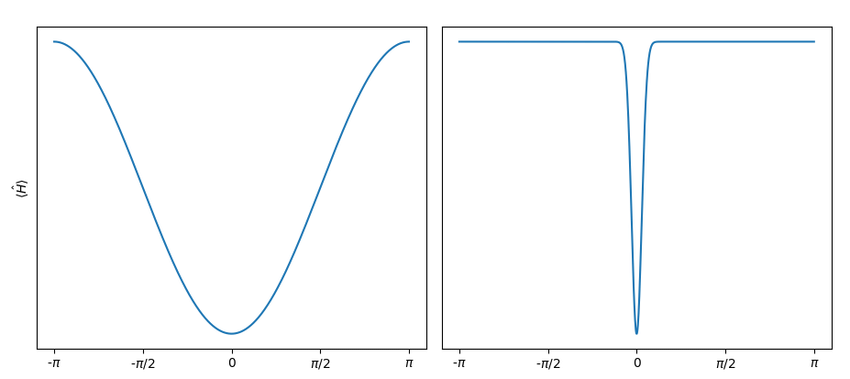
\includegraphics[width=\linewidth]{src/Appendices/example-of-a-barren-plateau.png}
    \caption{
        An illustrative example of a barren plateau and narrow gorge.
        On both plots: the expectation value of a Hamiltonian for a single parameter in the quantum circuit.
        On the left: expectation value landscape in the absence of barren plateau.
        On the right expectation value landscape in case of a barren plateau.
        Figure from Chen et al. \cite{tillyVariationalQuantumEigensolver2021}.
    }
    \label{fig: Barren Plateau Example}
\end{figure}

This research project undertakes a study that aims to survey and compare some countermeasure approaches to mitigate or avoid the effect of BP in the QNN development under VQA methods.
The main work of this article is summarized:
We provide some essential background for VQA and QNN;
We define the BP phenomenon and the causes that would lead to this issue;
The composition of known methods to address the matter of concern will be introduced, as well as performance comparison to identify the best approach;
Finally, we conclude the paper with some open issues and prospects for the field.
